\documentclass{abnt}

%Arquivo com os principais pacotes usados e suas descrições.

%%%%%%%%%%%%%%%%%%%%%%%%%%%%%%%%%%%%%%%%%
% 			Idiomas e Acentos			%
%%%%%%%%%%%%%%%%%%%%%%%%%%%%%%%%%%%%%%%%%
\usepackage[brazilian]{babel} % Habilita o uso do idioma português do brasil (PT-BR).
\usepackage[T1]{fontenc} 
%\usepackage{fontspec} % Habilita maior variedade de acentos. Pode ser necessario adicionar outros pacotes.
\usepackage{lmodern} % Habilita o uso da font Latin Modern.


%%%%%%%%%%%%%%%%%%%%%%%%%%%%%%%%%%%%%%%%%
% 				TABELAS					%
%%%%%%%%%%%%%%%%%%%%%%%%%%%%%%%%%%%%%%%%%
\usepackage{tabulary} % Cria tabelas mais facilmente.
\usepackage{booktabs} % Melhora o visual das tabelas.
\usepackage[table]{xcolor} % Pacote de cor pra as tabelas.
\usepackage{caption} % Melhora as legendas de imagens, tabela etc.

%%%%%%%%%%%%%%%%%%%%%%%%%%%%%%%%%%%%%%%%%
% 				IMAGENS					%
%%%%%%%%%%%%%%%%%%%%%%%%%%%%%%%%%%%%%%%%%
\usepackage{graphicx} % Facilita a inserção de imagens.


%%%%%%%%%%%%%%%%%%%%%%%%%%%%%%%%%%%%%%%%%
% 			CÓDIGO FONTE				%
%%%%%%%%%%%%%%%%%%%%%%%%%%%%%%%%%%%%%%%%%

%Documentação de código fonte.
\usepackage{listings}


%%%%%%%%%%%%%%%%%%%%%%%%%%%%%%%%%%%%%%%%%
% 	Símbolos e Caracteres Matemáticos	%
%%%%%%%%%%%%%%%%%%%%%%%%%%%%%%%%%%%%%%%%%
\usepackage{amsmath}
\usepackage{amssymb}
\usepackage{amsfonts}
\usepackage{mathspec} %Habilita o uso das fontes e dos caracteres matematicos.


%%%%%%%%%%%%%%%%%%%%%%%%%%%%%%%%%%%%%%%%%
%				ABNT					%
%%%%%%%%%%%%%%%%%%%%%%%%%%%%%%%%%%%%%%%%%
\usepackage[alf, abnt-etal-cite=2]{abntcite} % Ordena as referencias em ordem alfabética.
\usepackage{url} %Facilita o uso de url. Pode-se usar o comando \url{...}.


%%%%%%%%%%%%%%%%%%%%%%%%%%%%%%%%%%%%%%%%%
% 			Configurações				%
%%%%%%%%%%%%%%%%%%%%%%%%%%%%%%%%%%%%%%%%%
\captionsetup{justification=centering,labelfont=bf} %Formata a legenda das figuras.
%\graphicspath{{../imgs/}} %Define o diretorio padrão para buscar as imagens da apresentação.  
%\setromanfont[Ligatures=TeX]{Crimson}
%\defaultfontfeatures{Scale=MatchLowercase, Mapping=tex-tex}

%%%%%%%%%%%%%%%%%%%%%%%%%%%%%%%%%%%%%%%%%
%				BEAMER					%
%%%%%%%%%%%%%%%%%%%%%%%%%%%%%%%%%%%%%%%%%
%Define algumas configurações que serão validas para todo o documento.  
%\setbeamertemplate{section in toc}[sections numbered]
%\setbeamertemplate{subsection in toc}[subsections numbered]
%\setbeamertemplate{background canvas}[vertical shading][bottom=blue!3,top=blue!7]
%\setbeamertemplate{caption}[numbered]


%%%%% Dados para criação da capa e folha de rosto %%%%
\autor{	Denis F. de Carvalho,
		Guilherme A. de Macedo,
		Matheus L. Domingues da Silva e 
		Victor H. Carlquist da Silva
}
\titulo{Could Computing}
\orientador{Avelino Natal Bazanella Junior}
\comentario{Trabalho apresentado ao Prof. Avelino Bazanela Junior, na disciplina de Redes de Computadores
			presente no $2^{a}$ modulo do curso de Tecnologia em Análise e Desenvolvimento de Sistemas no IFSP-CJO.}
\instituicao{Instituto Federal de Educação, Ciência e Tecnologia de São Paulo -- \textit{campus} Campos do Jordão}
\local{Campos do Jordão}
\data{\today}

\begin{document}

	% Para utilizar o formato padrão de capa da ABNT, substituí o comando \maketitle pelo comando \capa.
	\capa
	
	\folhaderosto
	
	\begin{resumo}
		Este trabalho tem por objetivo mostrar e explicar o funcionamento da tecnologia de computação em nuvem (cloud computing). 
		A construção desse trabalho foi baseada em pesquisas em \textit{sites}, gráficos e tabelas, bem como a consulta de livros especializados.
	\end{resumo}

	\begin{abstract}
		This work aims to show and explain the workings of the technology Cloud Computing. The construction of this work was based on research on sites, graphs and tables and consultation of specialized books.
	\end{abstract}
	
	\sumario
	
	%\listadetabelas
	
	\listadefiguras
	
	\chapter{Introdução}
	
	A denominação \textit{cloud computing} chegou ao conhecimento de muita gente em 2008, 
	mas tudo indica que ouviremos este termo ainda por um bom tempo. Também conhecido no Brasil 
	como computação nas nuvens ou computação em nuvem, \textit{cloud computing} se refere, essencialmente, 
	à ideia de utilizarmos, em qualquer lugar e independente de plataforma, as mais variadas aplicações 
	por meio da internet com a mesma facilidade de tê-las instaladas em nossos próprios computadores.

	\chapter{O que é \textit{Cloud Computing} ?}

	Cloud Computing é um termo bastante utilizado hoje em dia. Significa, basicamente, 
	alocar recursos remotamente. Imagine que sua empresa necessitasse de um servidor de 
	arquivos e em tudo que isso acarretaria: você teria que contratar pessoal especializado, 
	ter um local na sua empresa para as máquinas, criar rotinas de backups, etc. 
	Enfim, você teria uma enorme dor de cabeça para conseguir configurar todo o servidor. 
	Utilizando o conceito de Cloud Computing você poderia simplesmente contratar um serviço na 
	internet onde você pagaria apenas pelo tanto que fizesse uso, não teria que se preocupar em 
	contratar pessoal especializado para a manutenção dos servidores, ou em ter um local na 
	sua empresa para as máquinas, nem criar rotinas de backups, ou seja, o servidor 
	estaria operacional em pouco tempo (apenas alguns cliques), apenas seria necessário 
	contratar o serviço e a empresa prestadora do serviço ficaria respondável por toda a 
	parte de configuração e manutenção do servidor.

	Podemos resumir os benefícios de se utilizar cloud computing em cinco conceitos:

    \begin{itemize}

        \item Espaço: todo o hardware ficará alocado na nuvem;

        \item Economia: você não precisará gastar com manutenção de hardware ou de software;

        \item Tempo: você só precisará de alguns cliques e tudo estará funcionando;

        \item Backup: a tarefa de backup e replicação dos dados fica por conta da empresa contratada;

        \item Configuração: Sem se preocupar com a disposição física dos servidores, 
        o usuário do serviço apenas acessaria as configurações básicas a respeito do mesmo.

    \end{itemize}

	\chapter{Por que surgiu?}

	O conceito de \textit{cloud computing} surgiu da necessidade de se terceirizar certos serviços 
	de informação dentro da empresa e da necessidade de os dados estarem sempre disponíveis 
	independente de onde esses dados estejam sendo acessados. Para uma empresa que não trabalha 
	com informática, ficaria muito caro e complexo criar e configurar vários tipos de servidores, 
	ela teria que criar um departamento inteiro só para cuidar da parte de informática 
	(banco de dados, servidor de arquivos, páginas web, etc). Já com \textit{Cloud Computing}, seria 
	necessário apenas contratar o serviço. Dentro da empresa ficariam apenas máquinas simples, 
	com poucos recursos, acessando os serviços na nuvem, independente de onde se esteja. Ou seja, 
	se sua empresa tem filiais, seria necessário apenas contratar um serviço e todas as filiais 
	compartilhariam o mesmo serviço. 

	\textit{Cloud Computing} pode funcionar com IaaS, PaaS ou SaaS, recursos, serviços ou softawares, 
	respectivamente, conforme explicado a seguir.

	\chapter{Modelos de Computação nas Nuvens}

	Com a utilização da computação em nuvem é possível oferecer o 
	hardware e o software como serviços. 
	Entre os diversos recursos disponiveis com a utilização dessa tecnologia, 
	destacam-se os metodos de SaaS, PaaS e IaaS.

	\section{SaaS}
	
	O \textit{Software} como serviço (\textit{Software as a Service} (SaaS)) é uma forma 
	de comercialização do \textit{software} pela internet. Nesse modelo, o fornecedor 
	fica responsável pela instalação, configuração e disponibilização do 
	software, e o usuário apenas paga pelo uso.
	Geralmente o acesso do usuário ao sistema é feito pela interface 
	de um navegador \textit{web}.

	\begin{figure}[h]
		\centering
		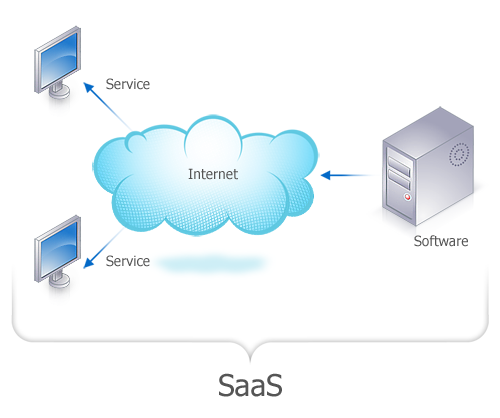
\includegraphics[width=10cm, keepaspectratio]{img/SaaS.png}
		\caption{Modelo SaaS.}
		\label{saas}
	\end{figure}
	
	Este modelo possibilita maior flexibilidade ao usuário, pois este não 
	precisa se preocupar como é feita a configuração do sistema em uso. Cabe 
	ao usuário apenas utilizar o serviço disponível.
	
	\section{PaaS}
		A Plataforma como Serviço (\textit{Platform as a Service} (PaaS)) possibilita a escolha rápida de recursos para desenvolvimento de aplicações.
		
		Esta plataforma é considerada a mais confusa das camadas do \textit{cloud}, geralmente sendo confundida com o SaaS ou IaaS (\textit{Infrastructure as a Service}).
		
		Uma plataforma na computação, se referindo ao \textit{software}, pode ser definida como os Sistemas Operacionais, por exemplo, Windows\texttrademark , Linux e Mac OS, e pode ser definida como os \textit{frameworks} para os aplicativos. Os SGBDs (Sistema de Gerenciamento de Banco de Dados) também estãos nesta camada.
	
		\begin{figure}[h]
			\centering
			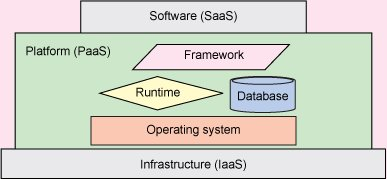
\includegraphics[width=8cm, keepaspectratio]{img/figure1.jpg}
			\label{fig_paas}
			\caption{Estrutura do PaaS}
		\end{figure}
		
		O que um bom provedor PaaS precisa ter:
			\begin{itemize}
		    \item Estrutura de desenvolvimento de aplicativo: Uma estrutura de desenvolvimento de aplicativo robusta desenvolvida em tecnologia amplamente usada, por exemplo, o Java;
            \item Disponibilidade: A plataforma de opção deve estar acessível e disponível em qualquer lugar, a qualquer hora;
            \item Escalabilidade: A plataforma deve ser inteligente o suficiente para aproveitar a capacidade elástica de uma infraestrutura;
            \item Segurança: Deve possuir dispositivos contra ataques;
            \item Inclusão: A plataforma deve fornecer a capacidade de incluir, embarcar e integrar outros aplicativos desenvolvidos nas mesmas plataformas ou em outras;
            \item Portabilidade: A plataforma deve permitir que as empresas movam o aplicativo de uma IaaS para outra.
		\end{itemize}
		
	\section{IaaS}
		Infraestrutura como Serviço (\textit{Infrastructure as a Service} (IaaS)) é a camada do \textit{Cloud Computer} de mais baixo nível. Ela pode ser defida como sendo a 'capacidade compucional' da nuvem. Ela é responsável pela infraestrura, ou seja, é nesta camada que se define a quantidade de processamento, de armazenamento, de memória RAM, etc. Toda esta estrutura pode ser encontrada em nossas casas, mas em escala muito menor. O IaaS trabalha nesse nicho, mas em escala industrial.
		
		O IaaS não é constituído por PCs(\textit{Personal Computer}), mas por diversos servidores robustos, e os dados ficam em \textit{storages}, que são máquinas que possuem grande contingência, poder de armazenamento e velocidade.
		
		Hoje em dia existem diversos serviços, que com apenas um clique pode se criar um servidor com a configuração que se deseja.
		
		O IaaS fornece seus serviços as outras duas camadas superiores, o PaaS e o SaaS.
		 
	\chapter{Possibilidades - Soluções disponíveis no mercado}

	\section{Solução de SaaS}

	\begin{itemize}
		\item[] Apple iCloud: A Apple lançou em 12 de outubro de 2011, o aplicativo chamado iCloud. Neste aplicativo os usuários apple podem 
	utilizar diversos recursos como os listados a seguir:
	\end{itemize}

	\begin{itemize}
	  \item iOS device backup and restore: Permite que usuários possam fazer \textit{backup} de seus dados diretamente na nuvem,
	  podendo acesa-los em qualquer lugar com acesso a internet;
	  \item Find My iPhone/Mac: Possibilita encontrar a localização de seu dispositivo utilizando a internet;
	  \item Find My Friends: Encontra seus amigos que também utilizam os serviços do \textit{iCloud};
	  \item Photo Stream: Qualquer foto tirada é compartilhada com todos os dispositivos cadastrados no \textit{iCloud};
	  \item Email: Serviço de email;
	  \item iTunes Match: Sincroniza as músicas do iTunes com todos os dispositivos cadastrados no \textit{iCloud}.
	\end{itemize}
	
	\section{Soluções de PaaS}

		\begin{itemize}
			\item Heroku: A plataforma Heroku permite hospedar aplicações \textit{web} escritas em diversas linguagens, como o Ruby, PHP, Java e outros. O serviço básico de hospedagem é gratuíto, mas com o uso de serviços do heroku, por exemplo, banco de dados, é cobrado uma taxa mensal.
			\item OpenShift - Red Hat: Esta plataforma permite hospedar aplicações em Java, PHP, Ruby e Python. Ela oferece dois tipos de serviços, um gratuíto e um pago. O serviço gratuíto é limitado, mas é possível hospedar diversos aplicativos, desde que não precise de banco de dados. Já o serviço pago possuí um poder de processamento melhor e suporte à banco de dados.
		\end{itemize}

	\section{Soluções de IaaS}

		\begin{itemize}
			\item Amazon Web Service (AWS): A AWS permite criar servidores na nuvem de acordo com a necessidade da empresa. É possível escolher a plataforma e o poder de processamento do servidor. Com apenas alguns cliques é possível criar esses servidores. 
			
			O AWS usa um sistema de cobrança chamado \textit{pay-as-you-go} (pague pelo uso, em tradução livre), isso significa que você só paga quando o serviço está ativo.
		\end{itemize}
	
	\chapter{Conclusão}
	
	Na verdade, qualquer tentativa de definir o que é \textit{cloud computing} pode não ser 100\% precisa. Isso porque as 
	ideias por trás da noção de computação nas nuvens são muito novas e as opiniões de especialistas em computação 
	ainda divergem. Mas a noção básica conseguimos adquirir com o acompanhamento dos trabalhos.
	
	É claro que ainda há muita coisa por fazer. Por exemplo, a simples ideia de determinadas informações ficarem 
	armazenadas em computadores de terceiros, mesmo com documentos garantindo a privacidade e o sigilo, 
	preocupam pessoas e, principalmente, empresas, motivo pelo qual este ponto precisa ser melhor estudado. 
	Além disso, há outras questões, como o problema da dependência de acesso à internet. Algumas companhias já 
	trabalham em formas de sincronizar aplicações \textit{off-line} com \textit{on-line}, mas tecnologias para isso ainda precisam 
	evoluir bastante.
	
	De qualquer forma, o futuro aponta para esse caminho. Companhias como Dell, Intel, Oracle e 
	Microsoft já estão trabalhando nas mais variadas soluções para \textit{cloud computing}.
	
	\bibliography{referencias}
	
\end{document}


